\documentclass[11pt]{article}
\usepackage[includeheadfoot, top=1.0in, bottom=1.0in, hmargin=1.0in]{geometry}
\usepackage[utf8]{inputenc}
\usepackage{fancyhdr}
\usepackage{url}
\pagestyle{fancy}
\usepackage{setspace}
\usepackage{tabularx}
\usepackage{graphicx}
\usepackage{caption}
\usepackage{subcaption}
\usepackage{hyperref}
\usepackage{multicol}

\usepackage{hyperref}
\hypersetup{
    colorlinks=true,
    linkcolor=blue,
    filecolor=magenta,      
    urlcolor=blue,
}


\lhead{Astronomy Lab II}
\rhead{Spring 2023}
\lfoot{Golant}
\rfoot{Tues 7-10pm}
\cfoot{\thepage}

\begin{document}

\begin{center}
\huge{Lab 5: Galaxies}\\ \medskip \Large{February 21, 2023}
\end{center}

%%%%%%%%%%%%%%%%%%%%%%% INTRO %%%%%%%%%%%%%%%%%%%%%%%
\section{Introduction: In a Galaxy Far, Far Away}
In the early 20th century, there was a strong tension amongst astronomers regarding the nature of some faint, fuzzy objects that could barely be resolved with a telescope. Some astronomers believed that these ``nebulae" were clusters of stars in our own Milky Way, while others believed that they were their own distant, independent islands of stars. This disagreement has since been deemed \textit{The Great Debate}. It wasn't until 1924 -- when Edwin Hubble measured the distance to one of these nebulae -- that astronomers were able to settle the debate: Hubble found the Andromeda ``nebula'' to be over \emph{2 million light years} away, confirming that this was indeed a \textbf{galaxy} far, far away (cue the Star Wars music).


\medskip
Since Hubble's discovery, astronomers have studied galaxies with great interest. Galaxies come in all shapes, sizes, colors, and luminosities.  Each of these properties can tell us something unique about a galaxy: we can learn about the stars and gas within the galaxy, or the amount of dark matter permeating the galaxy; we can learn about the age of the galaxy and its evolutionary history; and we can learn about the galaxy's surrounding environment and the interactions that this environment induces. The first step in understanding a galaxy is to determine what \emph{type} of galaxy it is -- and we can do this by just looking at it!  Today, we'll think about the \textit{morphology} (or shape and structure) of galaxies and what we can learn from that. The goals of today's lab are for you to get a sense of the diversity of galaxies in the Universe, to create and test a galaxy classification system of your own, and to learn what the morphology of a galaxy can tell us about its evolutionary state.

%%%%%%%%%%%%%%%%%%%%%%% MAKE YOUR OWN CLASSIFICATION %%%%%%%%%%%%%%%%%%%%%%%
\section{Classifying Galaxies}
\subsection{Make Your Own Classification System}
Navigate to \url{http://cas.sdss.org/dr7/en/proj/advanced/galaxies/classification.asp}; you should see a table with 3 columns (``Run,'' ``Camcol,'' and ``Field'').  Clicking on a number in the ``Field'' column will bring you to an image of one or more galaxies.

\noindent
\textbf{Complete the following in your lab write-up}:
\begin{enumerate}
    \item Look through each of the ``Field'' images and spend a little time thinking about the similarities and differences between each galaxy. Make a list of some characteristics or qualities that you might use to describe these galaxies.
    
    \item Come up with a method of \emph{classifying} these galaxies -- that is, how might you sort these galaxies into different, non-overlapping categories? Write out a series of steps (or create a diagram, like a flow chart or a branching hierarchy) detailing how you'd sort an arbitrary galaxy into the categories you came up with. (Note: there is no ``correct'' answer to this question, but do keep in mind that all the images are at different distances, so the \emph{perceived} brightness and size of these galaxies will be different from their actual brightness and size)
    
    \item Once you've finished crafting your classification system, find the Hercules Cluster image in the ``Lab 5'' folder (under ``Files'') on CourseWorks. 
    \begin{enumerate}
        \item Using your classification method from the previous question, classify each labeled galaxy.
        
        \item How robust is your system? Comment on what faults your method may have (if any).
        
        \item Would your classification method still work well when applied to images at different wavelengths? (say, images of the same galaxy in X-rays or radio waves)
    \end{enumerate}  


    \item Now, let's look at a few ``deep fields'' -- that is, images with \emph{very} many galaxies:
    \begin{itemize}
        \item The Hubble Ultra Deep Field: \url{https://cdn.spacetelescope.org/archives/images/large/heic0406a.jpg}

        \item The James Webb SMACS Deep Field: \url{https://webbtelescope.org/news/first-images/gallery/zoomable-image-deep-field-smacs-0723}

        \item The James Webb Pandora Deep Field: \url{https://webbtelescope.org/resource-gallery/images/zoomable-pandoras-cluster}
    \end{itemize}
    \begin{enumerate}
        \item With the exception of a few stars in these images, every object you see is a galaxy. Try to identify the stars. How did you identify them? (hint: stars imaged by James Webb look different from stars imaged by Hubble)

        \item Make a rough estimate of the number of galaxies in the Pandora Deep Field. Explain how you obtained this estimate. (Note: this image only covers one 15.6-\emph{millionth} of the whole sky)

        \item Do you see any weird galaxies in these images that don't neatly fit into your classification scheme? If so, describe these galaxies. How could you alter your classification scheme to include these galaxies?
    \end{enumerate}
\end{enumerate}

\subsection{Cue the Music: The Hubble Tuning Fork}

\noindent
Figure \ref{fig:Hubble} shows a simplified schematic of the galaxy classification system that we typically use in modern astronomy -- this diagram is known as the \textit{``Hubble tuning fork''} (or the ``Hubble classification system,'' or the ``Hubble sequence''). The Hubble sequence is a \emph{morphological} galaxy classification scheme introduced by Edwin Hubble in 1936 (the nickname of ``tuning fork'' comes from the shape in which this system is traditionally represented). Hubble's scheme divides galaxies into \emph{three} broad classes based on their visual appearance. \textbf{Answer the following in your lab write-up}:
\pagebreak
\begin{enumerate}
\setcounter{enumi}{4}
    \item There are three primary branches depicted on the tuning fork. 
    \begin{enumerate}
        \item What features distinguish each of the three branches from one another? (that is, how are the galaxies along one branch unique from the galaxies along the other two branches?)
        
        \item How do the galaxies \emph{within} each branch vary?
    \end{enumerate}
    
    \item How does the Hubble classification scheme compare with your galaxy classification system? 
\end{enumerate}

\begin{figure} [h!]
    \centering
    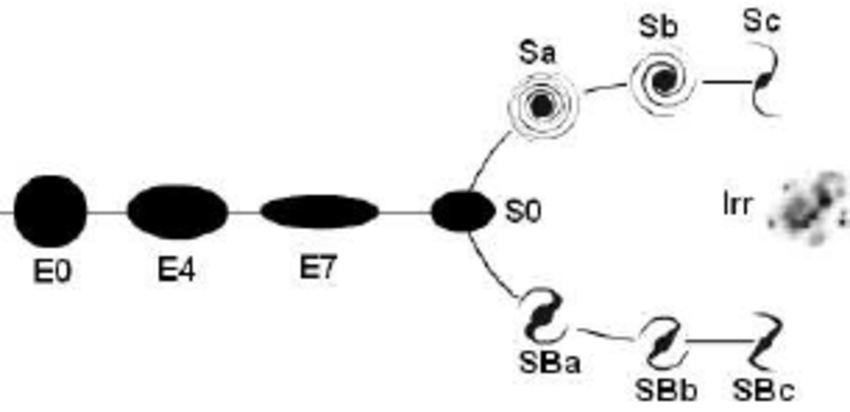
\includegraphics[width=0.7\textwidth]{Images/The-Hubble-tuning-fork.png}
    \caption{The Hubble tuning fork.}
    \label{fig:Hubble}
\end{figure}

\medskip


\noindent
You probably noted some of the following features in your description of the Hubble tuning fork; here are the formal names and descriptions for the galaxy types represented in Hubble's classification system:

\begin{itemize}
    \item \underline{Elliptical galaxies} (to the left of the tuning fork) appear as smooth, featureless ellipses in images. They are denoted by the letter `E,' followed by an integer `n' representing their degree of ``ellipticity'' (with $n=0$ being a spherical galaxy and $n=7$ being a very stretched-out ellipsoidal galaxy).
    
    \item \underline{Spiral galaxies} (to the right of the tuning fork) consist of a flattened ``disk'' with stars forming a spiral structure, along with a central concentration of stars known as the ``bulge,'' which is similar in appearance to an elliptical galaxy. Roughly half of all spirals are also observed to have a bar-like structure extending from the central bulge -- these ``barred spirals'' (on the bottom right of the tuning fork) are given the label `SB.' \emph{Unbarred} spiral galaxies (on the upper right of the tuning fork) are labeled with the letter `S.' 
    
    \item \underline{Lenticular galaxies} (at the center of the tuning fork) also consist of a bright central bulge surrounded by an extended disk-like structure -- but, unlike spiral galaxies, the disks of lenticular galaxies have no visible spiral structures and are not actively forming stars in any significant quantity. Lenticular galaxies are labeled `S0.'
    
    \item \underline{Irregular Galaxies} do not fit into the Hubble sequence, because they have no regular structure (neither disk-like nor ellipsoidal). Irregular galaxies are labeled `Irr.'
\end{itemize}
    

\medskip

%%%%%%%%%%%%%%%%%%%%%%% GALAXY ZOO %%%%%%%%%%%%%%%%%%%%%%%
\subsection{Galaxy Zoo}

Navigate to \url{https://www.zooniverse.org/projects/zookeeper/galaxy-zoo}. ``Galaxy Zoo'' is a citizen science project that invites amateur astronomers to help categorize large data sets of galaxy images. Once you're on the Galaxy Zoo main page, click ``Get Started" and read through the instructions; if you need some help, you can click on ``Need some help with this task?" or pull out the ``Field Guide" to the right of the screen. For the first galaxy you look at, I highly recommend reading through some of the examples under ``Need some help with this task?" 

\medskip \noindent
Classify 12 galaxies on Galaxy Zoo; as you're doing this \textbf{complete the following in your lab write-up}:
\begin{enumerate}
\setcounter{enumi}{6}
    
    \item Note anything unusual you see in the galaxies on Galaxy Zoo and how these factors might complicate both the Hubble classification system and your own classification system.

    \item Which shapes and types of galaxies are most common on Galaxy Zoo? (Note: the galaxies on Galaxy Zoo are \emph{very} far away)

    \item Your friend tells you that most of the galaxies in the Universe are elliptical.
    \begin{enumerate}
        \item Based on everything you've seen so far (Galaxy Zoo, the Deep Fields, the Hercules Cluster, etc.), defend or refute this claim. Be sure to cite specific evidence!
        \item Do you have enough evidence to definitively conclude that most of the galaxies in the Universe are elliptical? Why or why not? If not, what additional information would you need?
    \end{enumerate}
\end{enumerate}

\section{Galaxy evolution}
Look at the images labeled ``Coma'' and ``Abell 851'' in the ``Lab 5'' folder (under ``Files'') on CourseWorks. These two images show clusters of galaxies of similar density, but Abell 851 is more distant than Coma.
    \begin{enumerate}
    \setcounter{enumi}{9}
        \item Which of the two clusters has more elliptical galaxies?
        
        \item Given what you've seen earlier in the lab, are elliptical galaxies typically redder or bluer than spiral galaxies?
        
        \item Do redder main-sequence stars live longer or shorter than bluer main-sequence stars? Explain your reasoning. (\url{https://starinabox.lco.global/} may be useful)

        \item Are galaxies with lots of blue stars generally older or younger than galaxies with lots of red stars? Explain your reasoning.
        
        \item Based on the above information, what conclusions can you make about the Coma Cluster and Abell 851?
        
        \item Based on the above information, what generalizations can you make about the evolution of galaxies throughout the history of the Universe?
        \begin{enumerate}
            \item What additional information would help you make more robust generalizations about galaxy evolution?
        \end{enumerate}
    \end{enumerate}


%%%%%%%%%%%%%%%%%%%%%%% CONCLUSIONS %%%%%%%%%%%%%%%%%%%%%%%
\section{Wrapping Things Up}
\textbf{Answer the following questions in your lab write-up}:
\begin{enumerate}
\setcounter{enumi}{15}
    
    \item List some factors that make classifying galaxies a difficult task.

    \item How is galaxy morphology (i.e., galaxy shape) connected to the process of galaxy evolution?

    \item Given everything you've learned in this course so far -- about light, telescopes, spectroscopy, stars, and galaxies -- pose an open-ended question about stars and/or galaxies that could feasibly be answered with data. For example, you could ask ``On average, how many arms do spiral galaxies have?'' If you need some extra inspiration, you can scroll through the many beautiful images here: \url{https://esahubble.org/images/archive/category/galaxies/}. 
    
    \item If you have any additional questions, please post them on the Ed Discussion page. If you have some free time before next lab, please respond to at least one question (with either a follow-up question, a resource for further reading, or a full answer to the question).  
    
    \item If you have any feedback on how today's lab was run, or if you have any suggestions for future lab sessions, please let me know!
\end{enumerate}

\medskip
\noindent Note: There are many citizen science research projects like Galaxy Zoo that \emph{YOU} can participate in; each of these projects contribute to real research and will eventually result in published astronomy papers. Check out some of them here: \url{https://www.zooniverse.org/projects?discipline=astronomy&page=1&status=live}


\end{document}
